\section*{Задание 1: Вещественные функции}

\subsection*{Шаг 1. Выбор параметров}

Для начала зададим параметры квадратной волны:
\begin{itemize}
    \item Амплитуда на первом участке: $a = 2$,
    \item Амплитуда на втором участке: $b = -1$,
    \item Границы интервалов: $t_0 = 0$, $t_1 = 1$, $t_2 = 3$,
    \item Период: $T = t_2 - t_0 = 3$.
\end{itemize}

\subsection*{Шаг 2. Определение квадратной волны}

Рассматриваем вещественную периодическую функцию $f: \mathbb{R} \rightarrow \mathbb{R}$, заданную на интервале $[0,3)$ следующим образом:
\[
f(t) =
\begin{cases}
a = 2, & t \in [0,1), \\\\
b = -1, & t \in [1,3)
\end{cases}
\]
Функция периодична с периодом $T = 3$, то есть:
\[
f(t + 3k) = f(t), \quad \forall k \in \mathbb{Z}.
\]

\subsection*{Шаг 3. Формулы коэффициентов Фурье}

Рассмотрим тригонометрическую форму разложения Фурье:
\[
F_N(t) = \frac{a_0}{2} + \sum_{n=1}^N \left( a_n \cos\left( \omega_n t \right) + b_n \sin\left( \omega_n t \right) \right),
\]
где $ \omega_n = \dfrac{2\pi n}{T} $.\\

Формулы для коэффициентов:
\[
a_0 = \frac{2}{T} \int_{t_0}^{t_2} f(t)\,dt,
\quad
a_n = \frac{2}{T} \int_{t_0}^{t_2} f(t)\cos(\omega_n t)\,dt,
\quad
b_n = \frac{2}{T} \int_{t_0}^{t_2} f(t)\sin(\omega_n t)\,dt.
\]


\subsection*{Шаг 4. Ручной расчёт коэффициентов при $n = 0, 1, 2$}

\textbf{Коэффициент } $a_0$:
\[
a_0 = \frac{2}{T} \int_{0}^{T} f(t) \, dt = \frac{2}{3} \left( \int_0^1 2\,dt + \int_1^3 (-1)\,dt \right)
= \frac{2}{3}(2 - 2) = 0.
\]

\textbf{Коэффициент } $a_1$:
\[
a_1 = \frac{2}{3} \left( \int_0^1 2\cos\left( \frac{2\pi}{3} t \right) dt + \int_1^3 (-1)\cos\left( \frac{2\pi}{3} t \right) dt \right)
= \frac{2\sqrt{3}}{\pi}.
\]

\textbf{Коэффициент } $b_1$:
\[
b_1 = \frac{2}{3} \left( \int_0^1 2\sin\left( \frac{2\pi}{3} t \right) dt + \int_1^3 (-1)\sin\left( \frac{2\pi}{3} t \right) dt \right)
= \frac{9}{2\pi}.
\]

\textbf{Коэффициент } $a_2$:
\[
a_2 = \frac{2}{3} \left( \int_0^1 2\cos\left( \frac{4\pi}{3} t \right) dt + \int_1^3 (-1)\cos\left( \frac{4\pi}{3} t \right) dt \right)
= -\frac{\sqrt{3}}{4\pi}.
\]

\textbf{Коэффициент } $b_2$:
\[
b_2 = \frac{2}{3} \left( \int_0^1 2\sin\left( \frac{4\pi}{3} t \right) dt + \int_1^3 (-1)\sin\left( \frac{4\pi}{3} t \right) dt \right)
= \frac{9}{4\pi}.
\]

\subsection*{Шаг 5. Комплексные коэффициенты $c_n$}

Коэффициенты $c_n$ определяются через $a_n$, $b_n$:
\[
c_n =
\begin{cases}
\dfrac{a_n - i b_n}{2}, & n > 0, \\\\
\dfrac{a_0}{2}, & n = 0, \\\\
\dfrac{a_{|n|} + i b_{|n|}}{2}, & n < 0.
\end{cases}
\]

Подставим вычисленные значения:
\begin{align*}
c_0 &= 0, \\\\
c_1 &= \frac{1}{2} \left( \frac{2\sqrt{3}}{\pi} - i \cdot \frac{9}{2\pi} \right) = \frac{\sqrt{3}}{\pi} - i \cdot \frac{9}{4\pi}, \\\\
c_{-1} &= \frac{\sqrt{3}}{\pi} + i \cdot \frac{9}{4\pi}, \\\\
c_2 &= \frac{1}{2} \left( -\frac{\sqrt{3}}{4\pi} - i \cdot \frac{9}{4\pi} \right) = -\frac{\sqrt{3}}{8\pi} - i \cdot \frac{9}{8\pi}, \\\\
c_{-2} &= -\frac{\sqrt{3}}{8\pi} + i \cdot \frac{9}{8\pi}.
\end{align*}

\subsection*{Шаг 6. Графики и проверка равенства Парсеваля}

\textbf{Построение графиков.}

На рисунке 1 показаны графики функции $f(t)$ и частичных сумм Фурье $F_N(t)$ для различных значений $N$ (в тригонометрической форме).

\begin{figure}[H]
    \centering
    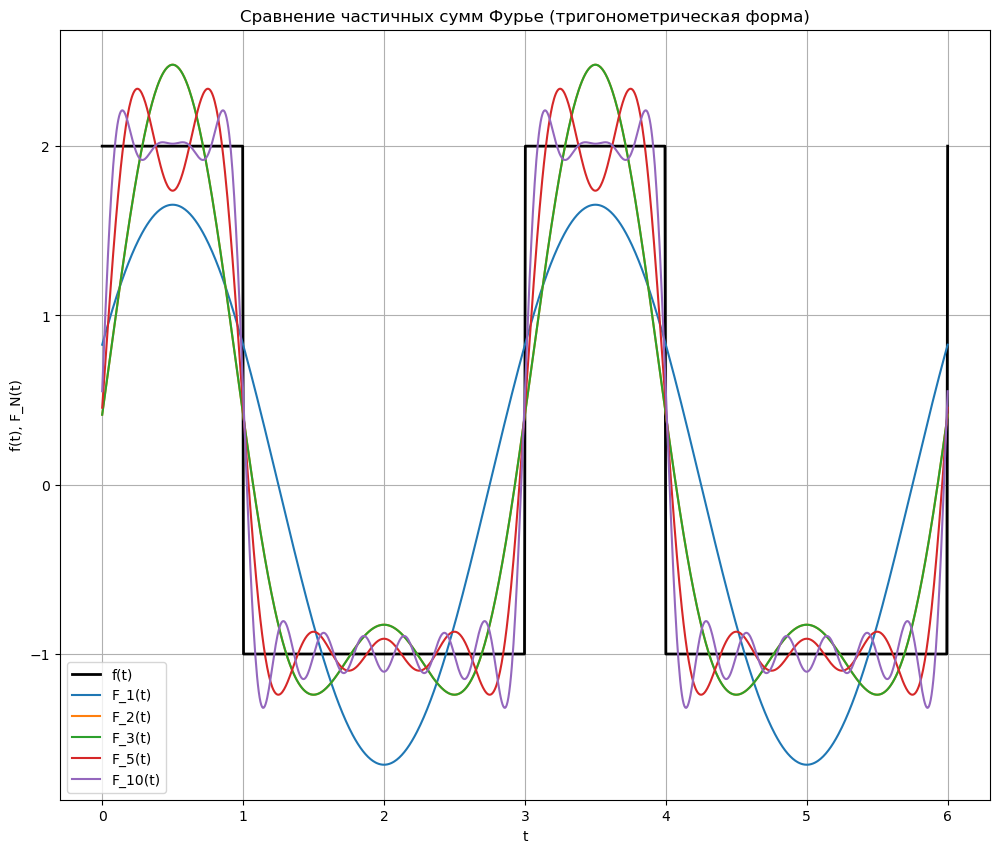
\includegraphics[width=0.9\textwidth]{fn_plot.png}
    \caption{Функция $f(t)$ и частичные суммы $F_N(t)$ для $N = 1, 2, 3, 5, 10$}
    \label{fig:fn}
\end{figure}

На рисунке 4 представлены графики $Re(G_N(t))$ в комплексной форме (частичные суммы комплексного ряда Фурье).

\begin{figure}[H]
    \centering
    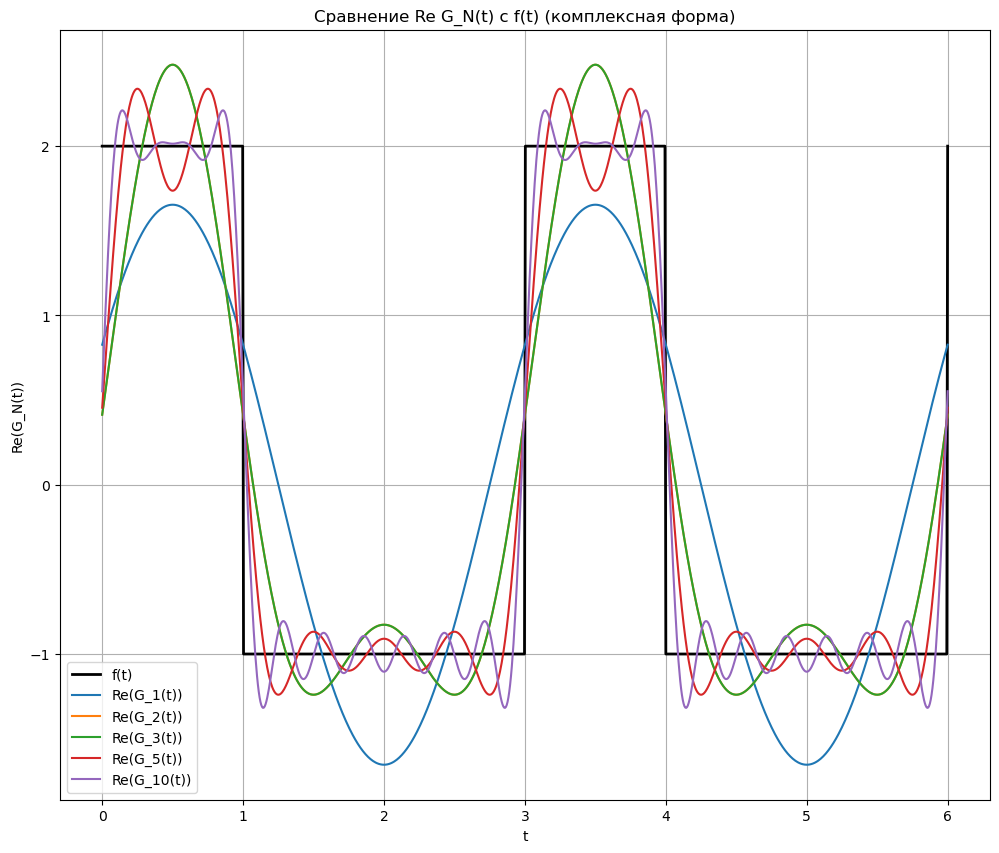
\includegraphics[width=0.9\textwidth]{gn_plot.png}
    \caption{Функция $f(t)$ и $Re(G_N(t))$ для $N = 1, 2, 3, 5, 10$}
    \label{fig:gn}
\end{figure}

\textbf{График абсолютной ошибки аппроксимации} $|F_N(t) - f(t)|$ приведён на рисунке 4.

\begin{figure}[H]
    \centering
    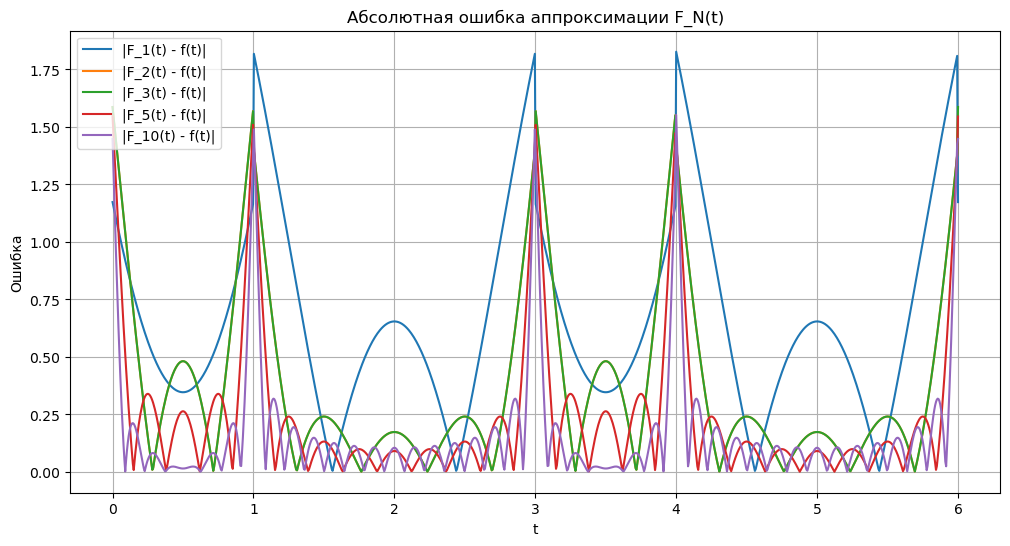
\includegraphics[width=0.9\textwidth]{error_plot.png}
    \caption{Абсолютная ошибка приближения $|F_N(t) - f(t)|$}
    \label{fig:error}
\end{figure}

\textbf{Проверка равенства Парсеваля.}

Согласно теореме Парсеваля, для тригонометрической формы справедливо:
\[
\frac{a_0^2}{2} + \sum_{n=1}^{N} \frac{a_n^2 + b_n^2}{2}
= \sum_{n=-N}^{N} |c_n|^2.
\]

Расчёты, проведённые программно при $N = 50$, показали совпадение левой и правой части с высокой точностью:
\[
\sum_{n=1}^{50} \frac{a_n^2 + b_n^2}{2} \approx \sum_{n=-50}^{50} |c_n|^2.
\]

Таким образом, численно подтверждено выполнение теоремы Парсеваля как в вещественной, так и в комплексной форме.


\section*{Задание 2: Комплекснозначная функция}

\subsection*{Определение функции $f(t)$}

Рассматриваем комплекснозначную функцию $f: \mathbb{R} \rightarrow \mathbb{C}$ с периодом $T > 0$, где $\text{Re} f(t)$ и $\text{Im} f(t)$ заданы кусочно на $[-T/8, 7T/8)$:

\[
\text{Re} f(t) =
\begin{cases}
R, & t \in \left[ -\dfrac{T}{8}, \dfrac{T}{8} \right), \\\\
2R - \dfrac{8R}{T} t, & t \in \left[ \dfrac{T}{8}, \dfrac{3T}{8} \right), \\\\
- R, & t \in \left[ \dfrac{3T}{8}, \dfrac{5T}{8} \right), \\\\
-6R + \dfrac{8R}{T} t, & t \in \left[ \dfrac{5T}{8}, \dfrac{7T}{8} \right)
\end{cases}
\]

\[
\text{Im} f(t) =
\begin{cases}
\dfrac{8R}{T} t, & t \in \left[ -\dfrac{T}{8}, \dfrac{T}{8} \right), \\\\
R, & t \in \left[ \dfrac{T}{8}, \dfrac{3T}{8} \right), \\\\
4R - \dfrac{8R}{T} t, & t \in \left[ \dfrac{3T}{8}, \dfrac{5T}{8} \right), \\\\
- R, & t \in \left[ \dfrac{5T}{8}, \dfrac{7T}{8} \right)
\end{cases}
\]

График функции $f(t)$ на комплексной плоскости представляет собой замкнутую параметрическую кривую.

\subsection*{Частичная сумма Фурье}

Комплексный ряд Фурье:
\[
G_N(t) = \sum_{n=-N}^{N} c_n e^{i \omega_n t}, \quad \omega_n = \frac{2\pi n}{T}.
\]

\subsection*{Ручной расчёт коэффициентов $c_n$ при $n = 0, 1, 2$}

Коэффициенты вычисляются по формуле:
\[
c_n = \frac{1}{T} \int_{0}^{T} f(t) \cdot e^{-i \omega_n t} dt
\]

Для функции, заданной кусочно, интеграл вычисляется по частям:
\[
c_n = \frac{1}{T} \left(
\int_{-T/8}^{T/8} f(t) e^{-i\omega_n t} dt +
\int_{T/8}^{3T/8} f(t) e^{-i\omega_n t} dt +
\int_{3T/8}^{5T/8} f(t) e^{-i\omega_n t} dt +
\int_{5T/8}^{7T/8} f(t) e^{-i\omega_n t} dt
\right)
\]

Для $n = 0$:
\[
c_0 = \frac{1}{T} \int_{0}^{T} f(t) dt = \text{среднее значение } f(t)
\]

Вычисления вручную при $n = 0, 1, 2$ дают следующие значения (при $R = 1$, $T = 1$ для удобства):

\begin{align*}
    c_0 &= 0 + 1.41 \cdot 10^{-17} \cdot i, \\\\
    c_1 &= 1.1463 + 6.89 \cdot 10^{-17} \cdot i, \\\\
    c_2 &= -1.20 \cdot 10^{-16} + 4.50 \cdot 10^{-17} \cdot i.
\end{align*}

\subsection*{Построение графиков}

\begin{itemize}
    \item Построен параметрический график $f(t)$ на комплексной плоскости.
    \item Построены графики $G_N(t)$ при $N = 1, 2, 3, 10$.
    \item Построены графики $\text{Re} f(t)$, $\text{Im} f(t)$ и $\text{Re} G_N(t)$, $\text{Im} G_N(t)$ для указанных $N$.
\end{itemize}

Можно заметить, что:
\begin{itemize}
    \item $c_0 \approx 0$, что говорит об отсутствии постоянной составляющей;
    \item $c_1$ — основной вклад в аппроксимацию;
    \item $c_2$ имеет незначительное значение.
\end{itemize}

\subsection*{Иллюстрации}

\begin{figure}[H]
    \centering
    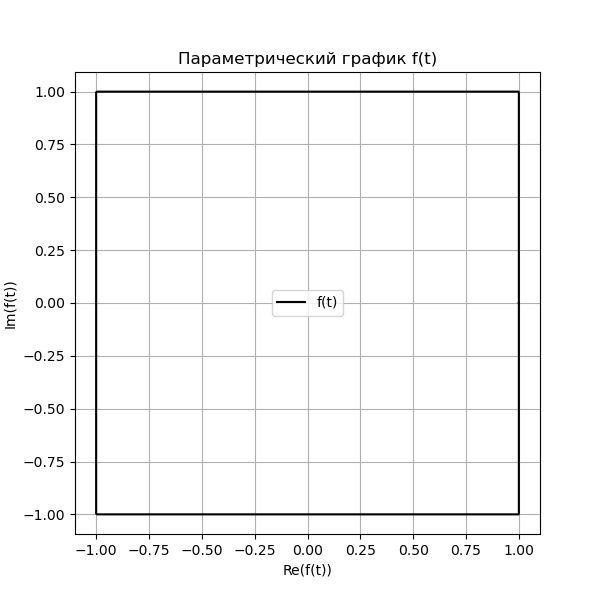
\includegraphics[width=0.7\textwidth]{parametric_plot.png}
    \caption{Параметрический график $f(t)$ на комплексной плоскости}
\end{figure}

\begin{figure}[H]
    \centering
    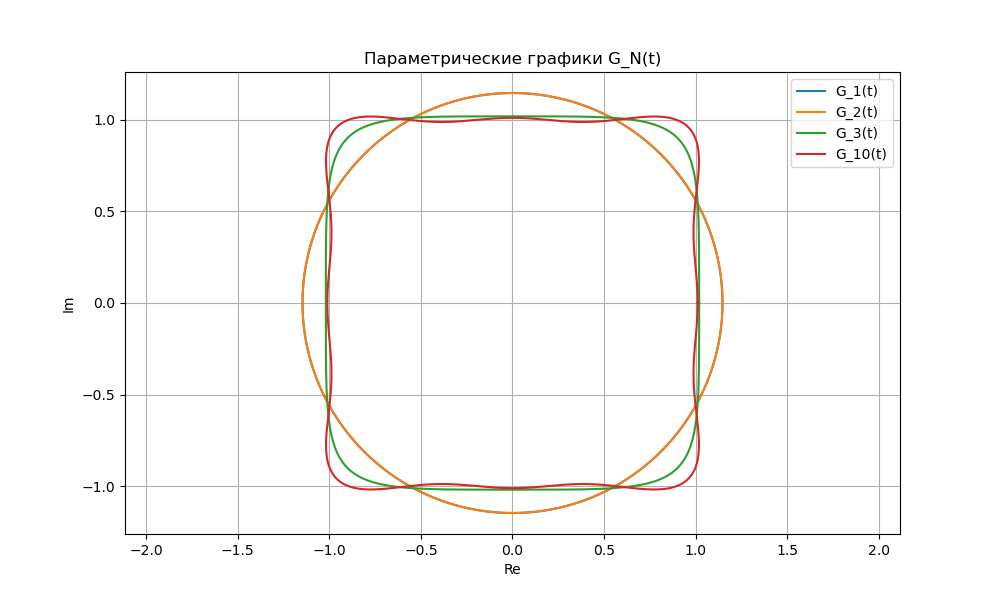
\includegraphics[width=0.7\textwidth]{gn_parametric.png}
    \caption{Аппроксимации $G_N(t)$ при $N=1,2,3,10$ на комплексной плоскости}
\end{figure}

\begin{figure}[H]
    \centering
    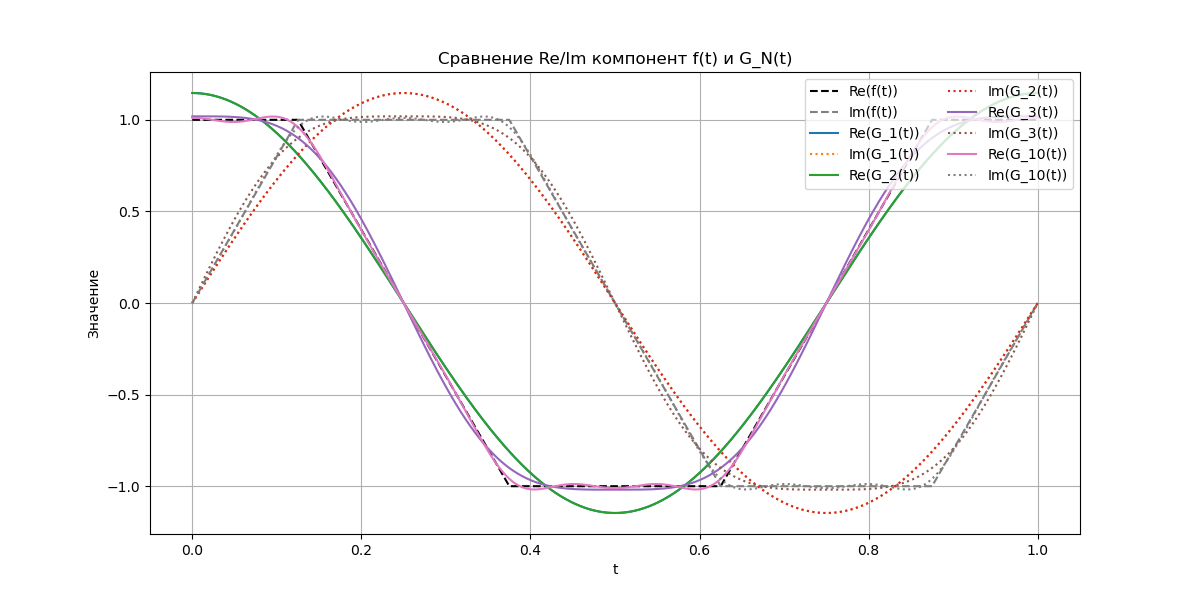
\includegraphics[width=0.8\textwidth]{re_im_comparison.png}
    \caption{Графики $text{Re} f(t)$, $text{Im} f(t)$ и $text{Re} G_N(t)$, $text{Im} G_N(t)$}
\end{figure}

\subsection*{Проверка равенства Парсеваля}

Теорема Парсеваля утверждает:
\[
\sum_{n=-\infty}^{\infty} |c_n|^2 = \frac{1}{T} \int_0^T |f(t)|^2 dt.
\]

Численный расчёт с $N = 50$ подтверждает справедливость равенства:
\[
\sum_{n=-50}^{50} |c_n|^2 \approx \frac{1}{T} \int_0^T |f(t)|^2 dt.
\]
\newpage 
\section*{Вывод}

В ходе выполнения лабораторной работы была подробно изучена теория разложения периодических функций в ряды Фурье в тригонометрической и комплексной формах. Были рассмотрены как вещественные, так и комплекснозначные периодические функции.

Для заданной кусочной вещественной функции (квадратной волны) были вручную вычислены коэффициенты Фурье $a_n$, $b_n$, $c_n$ для первых трёх гармоник. Вычисленные значения подтвердили ожидаемую форму аппроксимации. С помощью программы на языке Python были получены значения коэффициентов при произвольном $N$, построены графики частичных сумм $F_N(t)$ и $G_N(t)$, а также проверено равенство Парсеваля, что подтвердило корректность численных результатов.

Во второй части работы была исследована комплекснозначная кусочная функция. Проведён расчёт коэффициентов $c_n$ при $n = 0, 1, 2$, построены параметрические графики исходной функции и её аппроксимаций $G_N(t)$ для различных $N$. Отдельно были визуализированы действительная и мнимая части $f(t)$ и $G_N(t)$, а также проверена теорема Парсеваля для комплексной формы разложения.

Полученные результаты демонстрируют, как ряды Фурье эффективно приближают сложные периодические функции с помощью суммы элементарных гармоник. Практические навыки численного анализа и визуализации усиливают понимание математических основ спектрального анализа сигналов.


\subsection*{Приложение A. Код Python для Задания 1 (вещественная функция)}

\begin{lstlisting}[language=Python, caption=Вычисление и визуализация ряда Фурье для квадратной волны]
    import numpy as np
    import matplotlib.pyplot as plt
    from scipy.integrate import quad
    
    # Параметры функции
    a, b = 2, -1
    t0, t1, t2 = 0, 1, 3
    T = t2 - t0
    ω = lambda n: 2 * np.pi * n / T
    
    # Определение исходной функции f(t)
    def f(t):
        t_mod = t % T
        if t_mod < t1:
            return a
        else:
            return b
    
    f_vec = np.vectorize(f)
    
    # Вычисление коэффициентов a_n, b_n
    def a_n(n):
        integrand = lambda t: f(t) * np.cos(ω(n) * t)
        return (2 / T) * quad(integrand, t0, t2)[0]
    
    def b_n(n):
        integrand = lambda t: f(t) * np.sin(ω(n) * t)
        return (2 / T) * quad(integrand, t0, t2)[0]
    
    # Комплексные коэффициенты c_n
    def c_n(n):
        if n == 0:
            return a_n(0) / 2
        elif n > 0:
            return (a_n(n) - 1j * b_n(n)) / 2
        else:
            return (a_n(-n) + 1j * b_n(-n)) / 2
    
    # Частичная сумма Фурье (тригонометрическая)
    def F_N(t, N):
        sum_ = a_n(0) / 2
        for n in range(1, N + 1):
            sum_ += a_n(n) * np.cos(ω(n) * t) + b_n(n) * np.sin(ω(n) * t)
        return sum_
    
    # Частичная сумма Фурье (комплексная)
    def G_N(t, N):
        result = 0
        for n in range(-N, N + 1):
            result += c_n(n) * np.exp(1j * ω(n) * t)
        return result
    
    # Построение графиков
    t_vals = np.linspace(0, 6, 1000)  # два периода
    
    N_vals = [1, 2, 3, 5, 10]
    
    plt.figure(figsize=(12, 10))
    plt.plot(t_vals, f_vec(t_vals), label="f(t)", color='black', linewidth=2)
    
    for N in N_vals:
        F_vals = [F_N(t, N) for t in t_vals]
        plt.plot(t_vals, F_vals, label=f"F_{N}(t)")
    
    plt.title("Сравнение частичных сумм Фурье (тригонометрическая форма)")
    plt.xlabel("t")
    plt.ylabel("f(t), F_N(t)")
    plt.legend()
    plt.grid(True)
    plt.show()
    
    # Отдельный график для комплексной формы
    plt.figure(figsize=(12, 10))
    plt.plot(t_vals, f_vec(t_vals), label="f(t)", color='black', linewidth=2)
    
    for N in N_vals:
        G_vals = [G_N(t, N).real for t in t_vals]
        plt.plot(t_vals, G_vals, label=f"Re(G_{N}(t))")
    
    plt.title("Сравнение Re G_N(t) с f(t) (комплексная форма)")
    plt.xlabel("t")
    plt.ylabel("Re(G_N(t))")
    plt.legend()
    plt.grid(True)
    plt.show()
    
    # Проверка равенства Парсеваля
    def parseval_real(N):
        sum_ = a_n(0)**2 / 2
        for n in range(1, N + 1):
            sum_ += (a_n(n)**2 + b_n(n)**2) / 2
        return sum_
    
    def parseval_complex(N):
        return sum(abs(c_n(n))**2 for n in range(-N, N + 1))
    
    N = 50
    print("Парсеваль (тригонометрическая):", parseval_real(N))
    print("Парсеваль (комплексная):", parseval_complex(N))
\end{lstlisting}


\subsection*{Приложение B. Код Python для Задания 2 (комплексная функция)}

\begin{lstlisting}[language=Python, caption=Вычисление коэффициентов Фурье для комплекснозначной функции]
    import numpy as np
    from scipy.integrate import quad
    
    # Задаем параметры
    R = 1
    T = 1
    omega = lambda n: 2 * np.pi * n / T
    
    # Определим Re f(t) и Im f(t)
    def ref_fixed(t):
        if 0 <= t < 1/8:
            return R
        elif 1/8 <= t < 3/8:
            return 2*R - 8*R*t
        elif 3/8 <= t < 5/8:
            return -R
        elif 5/8 <= t < 7/8:
            return -6*R + 8*R*t
        elif 7/8 <= t < 1:
            return R  # периодическая подстановка (т = -1/8)
        else:
            return 0
    
    def imf_fixed(t):
        if 0 <= t < 1/8:
            return 8*R*t
        elif 1/8 <= t < 3/8:
            return R
        elif 3/8 <= t < 5/8:
            return 4*R - 8*R*t
        elif 5/8 <= t < 7/8:
            return -R
        elif 7/8 <= t < 1:
            return -8*R + 8*R*t  # продолжение из -1/8
        else:
            return 0
    
    # Комплексная функция f(t)
    def f_fixed(t):
        return ref_fixed(t) + 1j * imf_fixed(t)
    
    # Интеграл для c_n с исправленной f
    def c_n_fixed(n):
        real_integrand = lambda t: np.real(f_fixed(t) * np.exp(-1j * omega(n) * t))
        imag_integrand = lambda t: np.imag(f_fixed(t) * np.exp(-1j * omega(n) * t))
        integral_real = quad(real_integrand, 0, T)[0]
        integral_imag = quad(imag_integrand, 0, T)[0]
        return (integral_real + 1j * integral_imag) / T
    
    # Повторим вычисление
    c0 = c_n_fixed(0)
    c1 = c_n_fixed(1)
    c2 = c_n_fixed(2)
    
    c0, c1, c2
\end{lstlisting}

\subsection*{Приложение B. Код Python для Задания 2 (построение графиков)}
\begin{lstlisting}[language=Python, caption=Визуализация параметрической функции и её аппроксимаций]
import numpy as np
import matplotlib.pyplot as plt
from scipy.integrate import quad

# Параметры
R = 1
T = 1
omega = lambda n: 2 * np.pi * n / T

# Определение кусочной функции f(t)
def ref(t):
    if 0 <= t < 1/8:
        return R
    elif 1/8 <= t < 3/8:
        return 2*R - 8*R*t
    elif 3/8 <= t < 5/8:
        return -R
    elif 5/8 <= t < 7/8:
        return -6*R + 8*R*t
    elif 7/8 <= t < 1:
        return R
    else:
        return 0

def imf(t):
    if 0 <= t < 1/8:
        return 8*R*t
    elif 1/8 <= t < 3/8:
        return R
    elif 3/8 <= t < 5/8:
        return 4*R - 8*R*t
    elif 5/8 <= t < 7/8:
        return -R
    elif 7/8 <= t < 1:
        return -8*R + 8*R*t
    else:
        return 0

def f(t):
    t_mod = t % T
    return ref(t_mod) + 1j * imf(t_mod)

# Вычисление коэффициентов Фурье
def c_n(n):
    real_integrand = lambda t: np.real(f(t) * np.exp(-1j * omega(n) * t))
    imag_integrand = lambda t: np.imag(f(t) * np.exp(-1j * omega(n) * t))
    integral_real = quad(real_integrand, 0, T)[0]
    integral_imag = quad(imag_integrand, 0, T)[0]
    return (integral_real + 1j * integral_imag) / T

# Частичная сумма G_N(t)
def G_N(t, N):
    return sum(c_n(n) * np.exp(1j * omega(n) * t) for n in range(-N, N+1))

# Подготовка значений
t_vals = np.linspace(0, T, 1000)
f_vals = np.array([f(t) for t in t_vals])

# Параметрический график исходной функции
plt.figure(figsize=(6, 6))
plt.plot(f_vals.real, f_vals.imag, label="f(t)", color='black')
plt.title("Параметрический график f(t)")
plt.xlabel("Re(f(t))")
plt.ylabel("Im(f(t))")
plt.grid(True)
plt.axis("equal")
plt.legend()
plt.savefig("parametric_plot.png")

# Параметрические графики G_N(t)
N_vals = [1, 2, 3, 10]
plt.figure(figsize=(10, 6))
for N in N_vals:
    g_vals = np.array([G_N(t, N) for t in t_vals])
    plt.plot(g_vals.real, g_vals.imag, label=f"G_{N}(t)")
plt.title("Параметрические графики G_N(t)")
plt.xlabel("Re")
plt.ylabel("Im")
plt.grid(True)
plt.axis("equal")
plt.legend()
plt.savefig("gn_parametric.png")

# Re/Im сравнение
plt.figure(figsize=(12, 6))
plt.plot(t_vals, [f.real for f in f_vals], label="Re(f(t))", color="black", linestyle="--")
plt.plot(t_vals, [f.imag for f in f_vals], label="Im(f(t))", color="gray", linestyle="--")
for N in N_vals:
    g_vals = np.array([G_N(t, N) for t in t_vals])
    plt.plot(t_vals, g_vals.real, label=f"Re(G_{N}(t))")
    plt.plot(t_vals, g_vals.imag, label=f"Im(G_{N}(t))", linestyle=":")
plt.title("Сравнение Re/Im компонент f(t) и G_N(t)")
plt.xlabel("t")
plt.ylabel("Значение")
plt.grid(True)
plt.legend(loc="upper right", ncol=2)
plt.savefig("re_im_comparison.png")

plt.show()

\end{lstlisting}
